\chapter{Кубит как источник неклассического излучения}
Сверхпроводниковые кубиты обладают набором интересных свойств, которые позволяют контролируемым образом получить сильную связь квантовой системы и распространяющегося в волноводе поля без использования высокодобротных резонаторов. В частности, пример перспективной архитектуры для реализации микроволновой фотоники и электроники представляет схема, в которой единичный искусственный атом связывается с двумя полубесконечными линиями, которые не связаны друг с другом в отсутствии атома. При этом связь делается асимметричной. Это означает, что одна из линий, которую мы будем называть линией излучения, связана с кубитом сильным образом. Связь с линией излучения характеризуется константой распада $\Gamma_e\approx 2-20$~МГц, и она заведомо доминирует над остальными каналами распада и чистой дефазировки. Другая линия, которую мы будем называть линией контроля, размещается таким образом, что связь $\Gamma_c\ll\Gamma_e$ пренебрежимо мала. Однако, сильное поле в линии контроля может дать достаточную частоту Раби для быстрого возбуждения кубита, который сразу же начинает распадаться в линию излучения, таким образом создавая поле в этой линии. Одним из перспективных приложений таких систем может стать генерация неклассического распространяющегося света: например, успешно продемонстрирована генерация одиночных фотонов по требованию \cite{peng2016tuneable,Shaped_SPS,PechalShaped} и двух корреллированных и излучаемых в каскадном процессе фотонов, \cite{Wallraff_entangledPhotons}. В некоторых из этих работ в качестве перехода используется два нижних уровня потокового кубита, тогда как в других работах излучение идет с нижних уровней кубита-трансмона. Однако, остается открытым вопрос об возможности использования вышележащих уровней потокового кубита, шунтированного емкостью. 

В данном разделе мы расскажем о создании потокового кубита, асимметрично связанного с полупространствами, и изложим результаты просвечивающей спектроскопии, в которых успешно показано излучение на частотах различных кубитных переходов. Сравнивая результаты спектроскопических измерений с расчетными собственными энергиями кубитов, нам удалось восстановить картину энергетических состояний системы вплоть до третьего возбужденного уровня, что говорит о высокой степени контроля искусственного атома. Также при помощи измерения линии излучения удалось установить полную естественную ширину переходов $\ket{0}\leftrightarrows\ket{1}$ и $\ket{1}\leftrightarrows\ket{2}$ и увидеть расщепление Аутлера-Таунса при сильной накачке одного из переходов и измерении прохождения слабого пробного сигнала, настроенного на частоту другого перехода. Результаты данной работы составляют основу для разработки источников неклассического излучения микроволнового излучения на сверхпроводниковых искусственных атомах.
\section{Ассимметричная связь с двумя полупространствами}
Как было сказано выше, искусственный атом, исследуемый в данном разделе --- потоковый кубит, асимметрично связанный с двумя полубесконечными копланарными волноводами. Полезно представить оптический аналог такого размещения. Рассмотрим одиночный атом, подвешенный в трехмерном пространстве и расположенный позади крохотного отверстия, сделанного в непрозрачном экране. Предполагается, что размеры отверстия гораздо больше длины волны резонансного с атомным переходом света, поэтому при освещении экрана плоской монохроматической волной через отверстие проникают лишь экспоненциально затухающие т.н. \textit{эванесцентные} волны. Они распространяются лишь на расстояние порядка длины волны, но этого достаточно, чтобы возбудить атом за щелью. В свою очередь, возбужденный атом излучает поле в полупространство, свободное от экрана, где оно может быть задетектировано, отправлено в интерферометрическую схему или использовано в каких-либо других целях. Графическое изображение схемы представлено на Рис.~\ref{fig: hole}. 
\begin{figure}
	\centering
	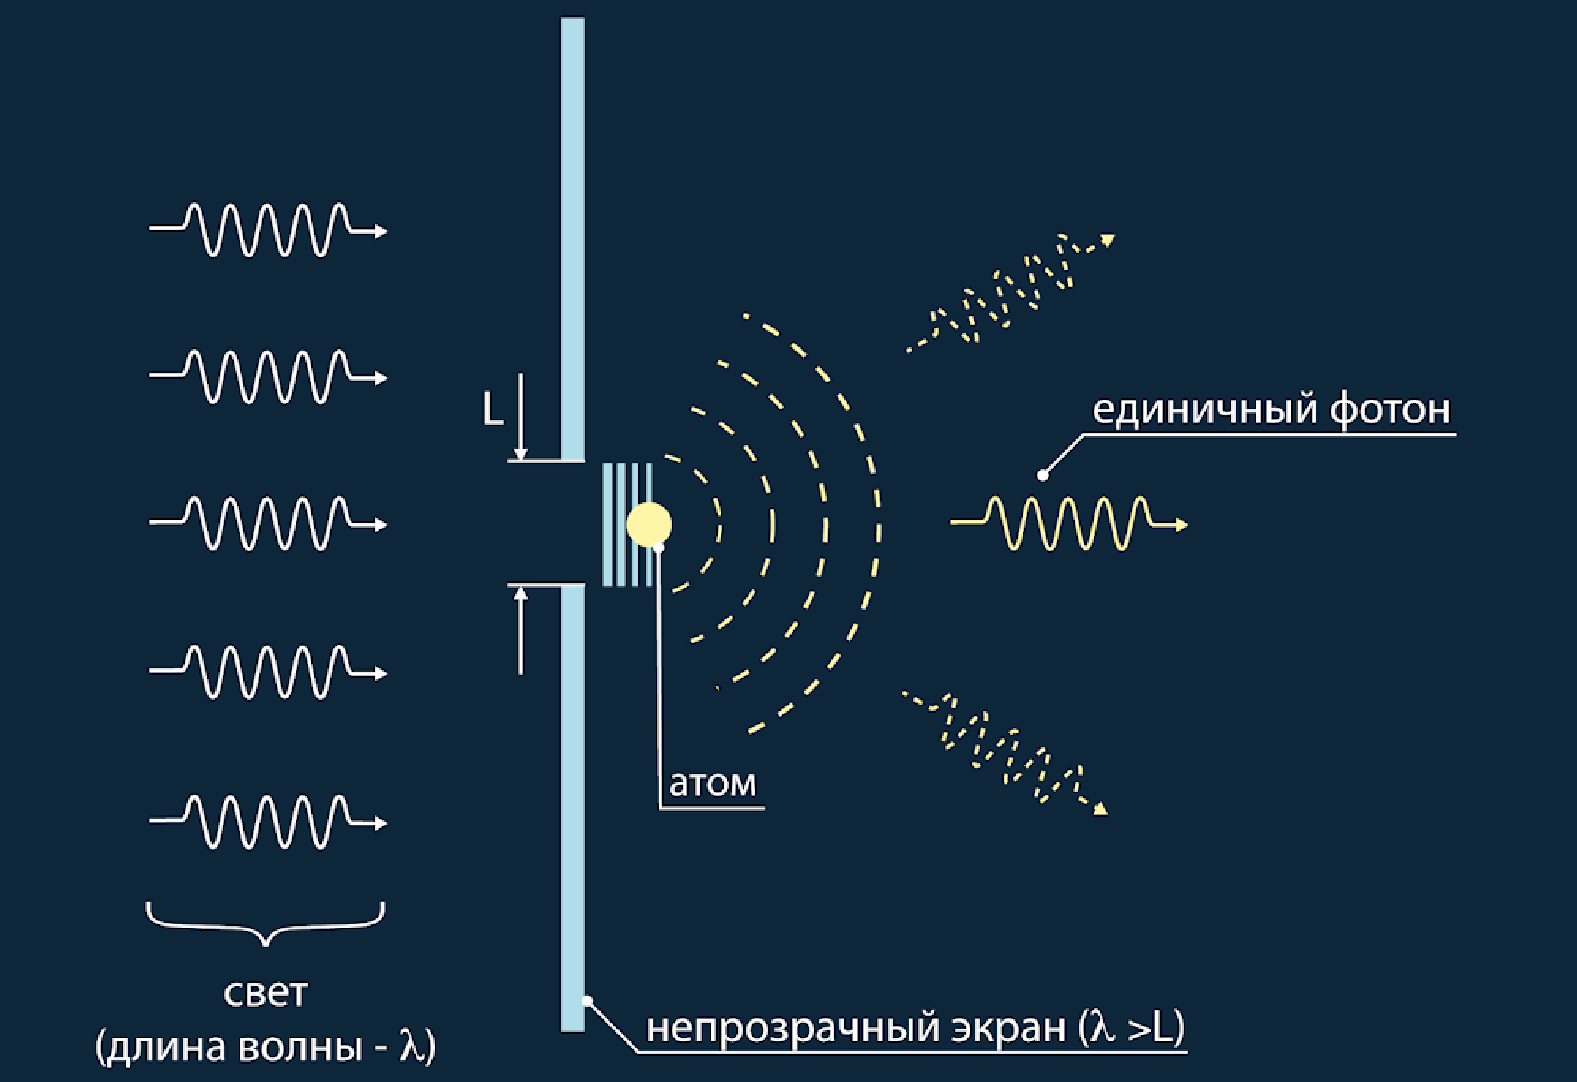
\includegraphics[width=0.85\textwidth]{sps_optical.pdf}
	\caption[Оптический аналог кубита, связанного с двумя полупространствами асимметричным образом]{Оптический аналог кубита, асимметрично связанного с двумя волноводами (подготовлено совместно с пресс-службой МФТИ). Непрозрачный экран с щелью шириной $L \ll \lambda$ образует два полупространства. Искусственный атом расположен вблизи щели справа от экрана. Плоская волна, падающая на экран слева, рассеивается на щели в виде эванесцентных волн, возбуждающих атом, который переизлучает в правое полупространство. В частности, таким образом можно осуществить генерацию одиночного фотона.}
	\label{fig: hole}
\end{figure}
Эквивалентная электрическая схема, где сверхпроводниковый потоковый кубит связан с полубесконечными волноводами, приведена на Рис.~\ref{fig: sps_scheme}(а). Емкость связи с линией контроля предполагается значительно меньшей, чем емкость связи с линией излучения. Как будет показано в следующем разделе, отношение этих емкостей является основным параметром, определяющим предельную эффективность кубита как источника одиночных фотонов. Отметим, что емкости $C_c$ и $C_e$ настолько малы, что эффективный импеданс между входной и выходной линией крайне велик и составляет порядка $10^3$ Ом. Поэтому классический импульс, налетающий слева, практически полностью отражается назад и не попадает в выходную линию. В свою очередь, в линии излучения (выходной линии) присутствует только поле, излучаемое атомом, поскольку связь атома и поля в правом волноводе достаточно сильная. 
\begin{figure}
	\centering
	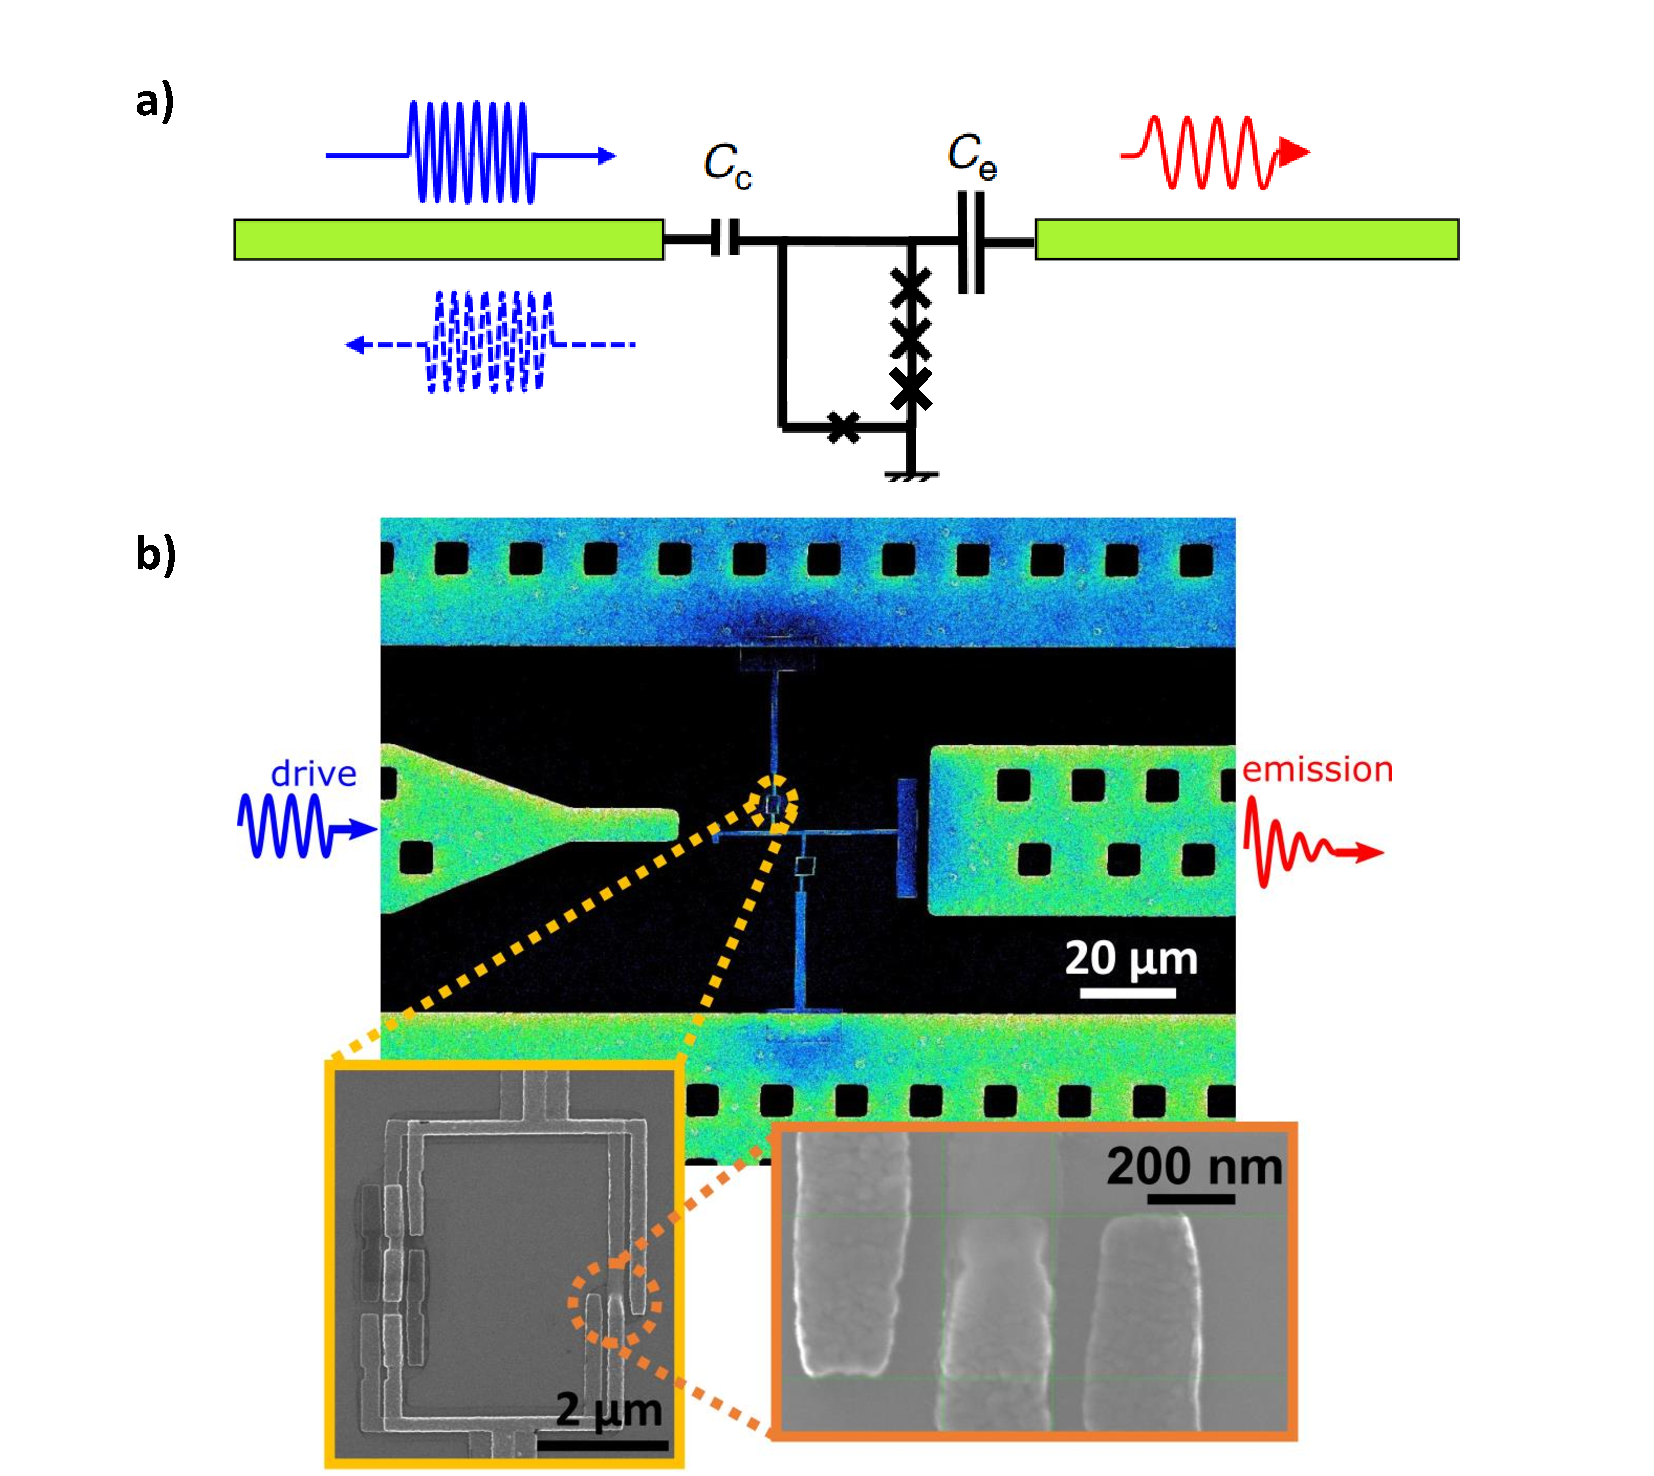
\includegraphics[width=1\textwidth]{SPS_schemes.pdf}
	\caption[Принципиальная электрическая схема и электронное изображение кубита, связанного с двумя полупространствами]{(a) - принципиальная электрическая схема потокового кубита, связанного с линией контроля при помощи емкости $C_c$ и линией излучения через емкость $C_e$. Классический управляющий сигнал (синяя волна) направляется в линию контроля и возбуждает атом, после чего он излучает в линию справа (красная волна). Схема адаптирована из \cite{peng2016tuneable} c разрешения авторов. (b) Изображение экспериментального образца кубита в сканирующем электронном микроскопе.}
	\label{fig: sps_scheme}
\end{figure}
В следующем разделе мы подробно рассмотрим параметры экспериментального образца кубита, используемого для наблюдения многоуровневой спектроскопии атома через линию излучения.
\section{Дизайн и параметры прибора}
Наш прибор представляет собой потоковый сверхпроводящий кубит с четыремя джозефсоновскими переходами \cite{Astafiev2010resonance,qiu2016four}, сфабрикованный при помощи стандартной методики двухуглового теневого напыления, см. Рис.~\ref{fig: sps_scheme}(b). Размеры трёх больших переходов одинаковы и равны $0.2\times0.8$~$\mu m $, а четвёртый в $\alpha \approx 0.35$ раз меньше по площади.  Один конец $\alpha$-перехода заземлён, а другой связан с линиями передачи. Входная линия присоединена к атому через небольшую ёмкость $C_i\approx0.5$~фФ, а большая ёмкость $C_e\approx2.8$~фФ соединяет атом и считывающую линию. Тогда эффективная ёмкость $\alpha$-перехода является суммой его собственной ёмкости $C_\alpha \approx 2.5$~fF  и двух связывающих ёмкостей ($C_\alpha + C_i + C_e$). Величина незатухающего тока $I_p=18$~nA в петле меньше, чем в обычных потоковых кубитах, что делает его менее чувствительным к шуму магнитного поля. Это приводит к значительному увеличению времени дефазировки \cite{yan2016flux}, но уменьшает ангармонизм уровней кубита, как и в кубитах типа трансмон \cite{koch2007charge}. Полученной в наших экспериментах величины ангармонизма порядка $1.5$~ГГц достаточно для сохранения верности двухуровневого приближения, даже на высоких возбуждающих мощностях. В то же время, более высокие уровни $\ket{2}$ and $\ket{3}$ сдвигаются вниз по энергии, так что частоты $\ket{1} \leftrightarrow \ket{2}$ and $\ket{2} \leftrightarrow \ket{3}$ оказываются в полосе работы HEMT-усилителей (1-12 ГГц), и переходы могут быть изучены напрямую.
\section{Описание схемы эксперимента}
Для измерений образец загружается в держатель с микроволновыми копланарными линиями. Держатель присоединяется к нижней части криостата растворения Bluefors-LD250 и охлаждается до температуры 15 мК. При такой температуре $k_B T \ll \hbar \omega_{01}$, и атом находится в невозбуждённом состоянии $\ket{0}$. Сильная связь между атомом и выходной линией достигается, если частота безызлучательного перехода $\Gamma_{\text{NR}}$ состояния $\ket{1}$ много меньше естественной ширины линии $\Gamma^{01}_{1}$, обусловленной преимущественно спонтанной эмиссией в считывающую линию. В эксперименте, отличном от нашего: одиночный атом в линии передачи \cite{Astafiev2010resonance,Delsing2013microwave1Dspace} --- это выражается в практически полном отражении достаточно слабой микроволновой волны с частотой $\omega$, близкой к $\omega_{01}=(E_1 - E_0)/\hbar$: коэффициент отражения $r$ может достигнуть единицы, если $\omega = \omega_{01}$, однако далеко от резонанса $r$~=~0. Это означает, что свет может полностью рассеяться на одиночной квантовой системе. В нашей схеме с асимметричной связью атома с двумя полупространствами резонансное возбуждение приходит со стороны входной линии. Излучение возбуждённого кубита может уйти в любую из линий, однако, как это было показано в \cite{peng2016tuneable}, переизлучение происходит в считывающую линию с эффективностью $1-C^2_{i}/C^2_{e} \approx$~0.97 в случае отсутствия безызлучательной составляющей и дефазировки. В теории, за счёт увеличения отношения ёмкостей эффективность может быть сколь угодно близкой к единице. Тогда наша система будет работать как источник одиночных микроволновых фотонов, если подать на вход возбуждающий $\pi$-импульс.
В наших экспериментах мы изучаем также другое свойство нашей системы: когерентное излучение атома. Так как входная и выходная линии слабо связаны друг с другом из-за рассогласования импедансов: $|Z_s| = 1/\omega_{01} C_{i} \approx 6 \cdot10^4$~Ом много больше импеданса линии $Z_0=50$~Ом --- подавляющая часть входной мощности отражается назад. Поэтому состояние поля в считывающей линии будет определяться тем, что излучает атом. Так как наш искусственный атом --- одиночная квантовая система, то и излучаемое поле в общем случае существенно неклассическое. Соответственно, изучение спектра и интенсивности когерентных излученных волн позволяет извлекать информацию об уровнях энергии искусственного атома. Для детектирования амплитуды и фазы когерентного излучения атома используется ВАЦ, выход которого через гетеродинную схему подключен к входной линии, а вход подключен к линии излучения.

\section{Многоуровневая спектроскопия источника}
Спектроскопические измерения начинаются с того, что мы находим частоту перехода $\ket{0} \leftrightarrow \ket{1}$, подавая на нашу систему микроволновый сигнал на частоте $\omega$, изменяемой в широком диапазоне, и меряя пропускание системы. Также мы меняем магнитное поле через петлю потокового кубита. На Рис.~\ref{spectr}a) изображён типичный спектр: интенсивность на выходе из системы, измеренная при помощи ВАЦ, как функция внешнего поля и частоты возбуждающей гармоники. Максимальная интенсивность на выходе из атома определяется его однофотонной мощностью излучения $P_{01}=\hbar\Gamma^{01}_1 \omega_{01}$, которая, в свою очередь, ограничена скоростью излучения $\Gamma^{01}_1$: двухуровневая система не может излучать более чем один фотон за раз. Соответствующая максимальная входная мощность, которую рассеивает кубит, равна $P \sim P_{01} \sim 10^{-17}$~Вт. Светлая линия на Рис.~\ref{spectr}a) соответствует низшему переходу $\ket{0} \leftrightarrow \ket{1}$; такая методика позволяет обнаружить только этот переход из-за высокого ангармонизма кубита.
\begin{figure*}[htb] 
	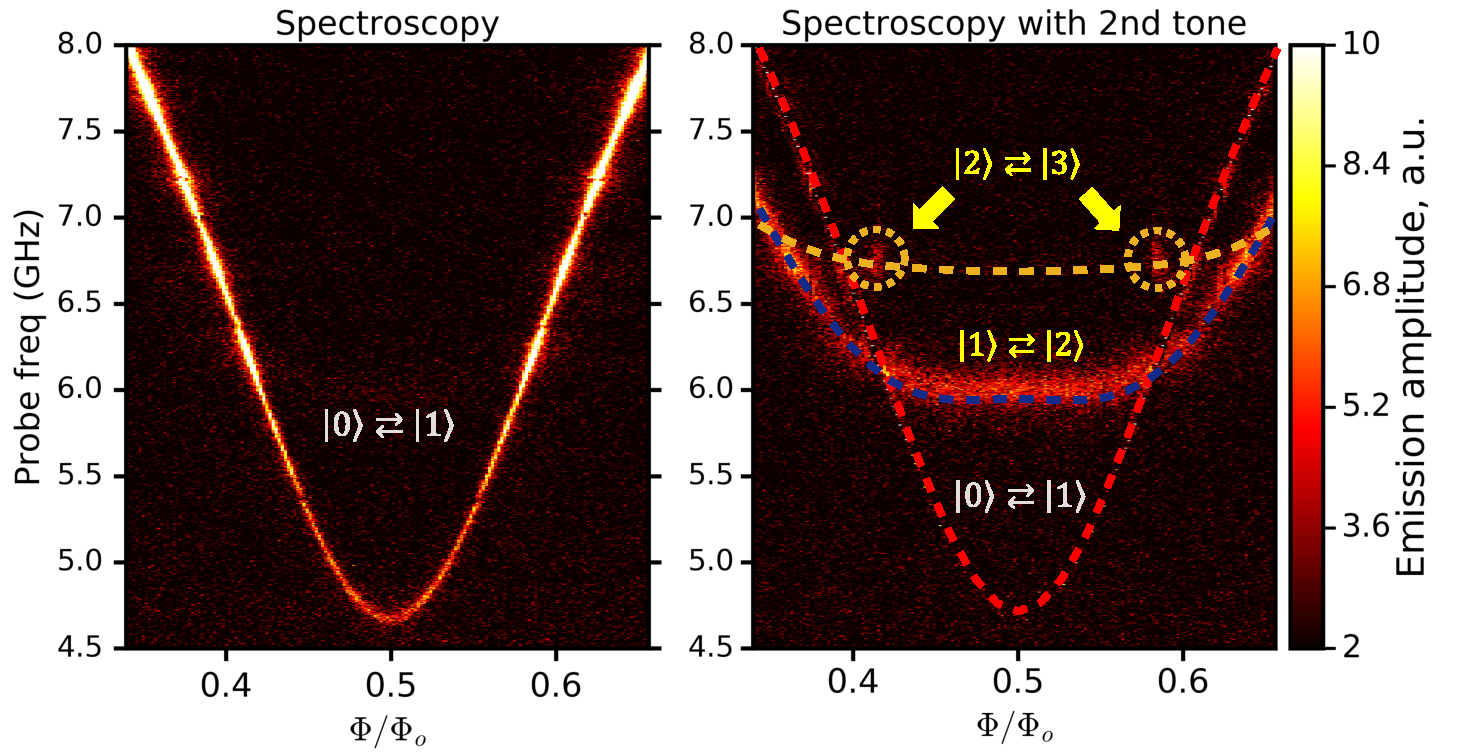
\includegraphics[width=1\textwidth]{figure_2-1} 
	\caption{Спектроскопия системы. Амплитуды излучения, измеренные с помощью VNA, как функции частоты возбуждающего поля и магнитного потока $\Phi$ через петлю кубита. (a) Напрямую измеренный переход $\ket{0}\leftrightarrow \ket{1}$. (b) Переход $\ket{1}\leftrightarrow\ket{2}$, измеренный, когда первый уровень $\ket{1}$ (красная пунктирная кривая) возбуждён приложением первого тона на частоте $\omega_{01}$. Пунктирные кривые - это численно рассчитанные уровни потокового кубита с параметрами нашего образца. Помимо этого, когда $\omega_{01}=\omega_{12}$, уровень $\ket{2}$ заселён, и видно излучение от перехода $\ket{2}\leftrightarrow\ket{3}$ (внутри жёлтых кругов)   }
	\label{spectr}
\end{figure*}
Далее, мы предлагаем метод измерения переходов между более высокими уровнями. Например, для измерения перехода $\ket{1} \leftrightarrow \ket{2}$ мы облучаем атом двумя синусоидальными сигналами: одним на частоте $\omega_{01}$ с увеличенной мощностью $\sim10^{-13}$~Вт и вторым низкой мощности $\sim P_{01}$. При этом, частота второго сигнала меняется в том же диапазоне, что и на Рис.~\ref{spectr}a. Первый сигнал насыщает состояния $\ket{0}$ и $\ket{1}$ атома до приблизительно 50\%. В такой схеме, второй сигнал может перевести атом из состояния $\ket{1}$ в $\ket{2}$, а атом начнёт излучать сигнал с частотой $\omega_{12}=(E_2 - E_1)/h$. Это подтверждается на эксперименте: на Рис.~\ref{spectr}b видна дополнительная спектральная линия, соответствующая переходу $\omega_{12}=(E_2 - E_1)/h$. Два ярких пятна на $\Phi \approx 0.42 \Phi_0$ и $\Phi \approx 0.58 \Phi_0$ (где $\Phi_0$ - квант магнитного потока) мы объясняем возбуждением уровня $\ket{3}$ системы, потому что в указанных значениях магнитного потока частота перехода $\ket{0} \leftrightarrow \ket{1}$ совпадает с частотой перехода $\ket{1} \leftrightarrow \ket{2}$. Это позволяет заселить состояние $\ket{2}$ первым тоном, в то время как второй тон при соответствии частот может заселить уровень $\ket{3}$, что и выражается в наблюдении излучения на частоте перехода $\ket{3} \leftrightarrow \ket{2}$.
\begin{figure}[tbh] 
	\centering
	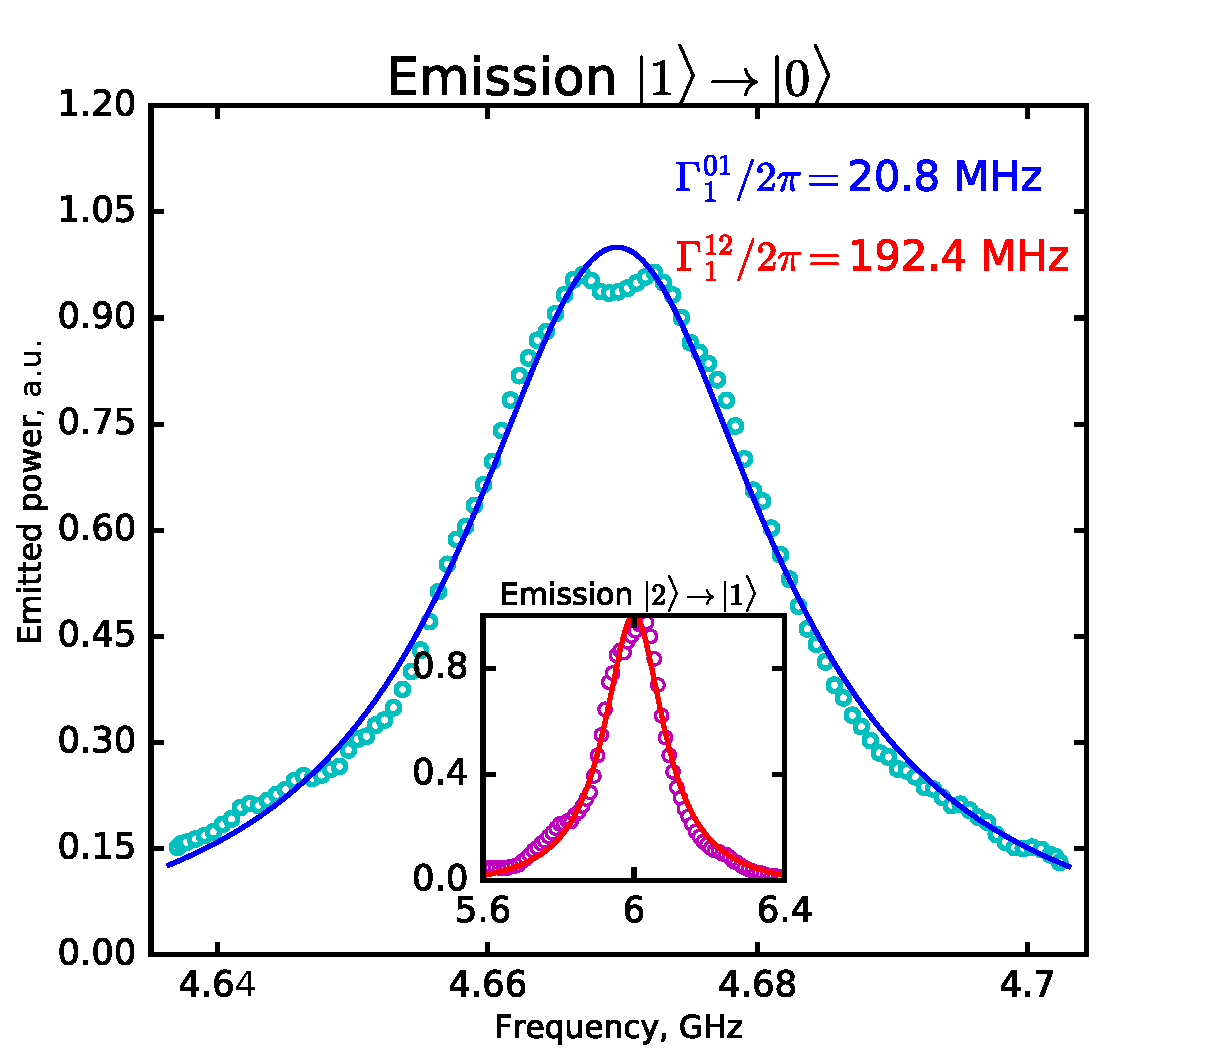
\includegraphics[width=0.7\columnwidth]{figure_3-1} 
	\caption{Интенсивность когерентного излучения системы как функция входной частоты. Искусственный атом облучается монохроматическим внешним сигналов, при этом измеряется мощность упруго рассеянного света. В случае малой мощности, переход $\ket{i} \leftrightarrow \ket{j} $ имеет форму лоренциана \cite{Astafiev2010resonance} с полной шириной на половине высоты, равным $\Gamma^{ij}_1$.
	}
	\label{peaks}
\end{figure}
Из спектроскопии системы можно извлечь другие её параметры: например, времена релаксации. На Рис.~\ref{peaks} изображена зависимость коэффициента пропускания от частоты в точке вырождения по магнитному полю ($\Phi = \Phi_0/2$). Коэффициент пропускания $\ket{0}\leftrightarrow \ket{1}$ изображён на синей кривой, $\ket{1}\leftrightarrow\ket{2}$ - на красной кривой во вставке. После фитирования их лоренцианом
\begin{equation}
	P(\omega)=\frac{1}{\pi}\frac{\Gamma/2}{(\omega-\omega_0)^2+\left(\Gamma/2\right)^2},
\end{equation} 
мы извлекаем значения скоростей распада $\Gamma_{1}^{01}/2\pi=20.8$~МГц and $\Gamma_{1}^{12}/2\pi=192.4$~МГц. Эти значения позволяют, в частности, получить уже использованное значение однофотонной мощности $P_{01} \sim 10^{-17}$~Вт. Как уже было сказано, скорость перехода между произвольными состояниями атома определяется скоростью излучения в считывающую линию и может быть рассчитана, если все параметры системы известны \cite{Astafiev-quantum-amplifier,Astafiev2010resonance}.

Теоретически рассчитанный спектр системы получается из диагонализации гамильтониана четырёх джозефсоновских переходов в зарядовом базисе. Результат приведён на Рис.~\ref{spectr}b (пунктирные кривые). Спектры расссчитаны для параметров: $E_J/2\pi=35$, $E_{Cc}/2\pi=13.5$, $E_C/2\pi=19$~ГГц и $\alpha=0.31$.  Видно, что расчет отлично согласуется с экспериментом. Зарядовая энергия связи обозначена как $E_{cC} = 4e^2/2(C_c+C_e+C_s)$, где $C_s$ --- некоторая емкость на землю, в то время как $E_C$ --- зарядовая энергия каждого из больших джозефсоновских переходов. На том же рисунке приведена теоретическая кривая для перехода  $\ket{2} \leftrightarrow \ket{3}$. Как было указано ранее, в эксперименте излучение на частоте этого перехода наблюдается только при некоторых значениях потока.
После проведения спектроскопического эксперимента опишем, как исследуемый образец может быть использован в качестве источника одиночных фотонов. Для этого рассчитаем коэффициенты прохождения и отражения В аналогичной разделу \ref{sec: scatt} манере рассмотрим рассеяние поля, идущего на кубит из линии контроля либо из линии излучения, и определим коэффициенты отражения и прохождения в зависимости от частоты Раби, констант связи, дефазировки и отстройки частоты внешнего поля от частоты кубита.
\section{Эффективность прибора в качестве источника одиночных фотонов}
Для полной характеризации коэффициентов прохождения и отражения непрерывных волн достаточно использовать выражение \eqref{eq: stat_s-}, при этом нужно помнить, что стационарное состояние зависит от полной релаксации $\Gamma_1 = \Gamma_1^c + \Gamma_1^e + \Gamma_1^{\text{nr}}$. С учетом этого выражения, среднее поле в линии контроля и в линии излучения \cite{peng2016tuneable} можно вычислить следующим образом:
\begin{subequations}\label{coherentwaves}
	\begin{eqnarray}
		&x < 0: &V_{c}(x,t)=i\frac{\hbar\Gamma_1^{c}}{C_{c} \nu_{a}}\langle\sigma^{-}\rangle e^{-i\omega t - ikx}, \\
		&x > 0:  &V_{e}(x,t)=i\frac{\hbar\Gamma_1^{e}}{C_{e} \nu_{a}}\langle\sigma^{-}\rangle e^{-i\omega t + ikx},
	\end{eqnarray}
\end{subequations}
где $\nu_a$ --- атомный дипольный момент перехода 0-1. 
Из этих уравнений легко получить выражения для коэффициента отражения поля в контрольной линии $r_{\text{c}}$ и коэффициента прохождения в линию линии излучения $t_{\text{ce}}$. Однако, для определения внутренних потерь наиболее подходящим измерением является зависимость коэффициента отражения поля, направленного на кубит через линию излучения $r_{\text{e}}$, от отстройки $\delta\omega$, которая для случая $\Omega^2\ll\Gamma_1\Gamma_2$ выражается соотношением:
\begin{eqnarray}
	&r_e& = 1-\frac{\Gamma_1^e}{\Gamma_2}\frac{1}{1-i\delta\omega/\Gamma_2}.\label{re}
\end{eqnarray}
\begin{figure}[!h]
	\centering
	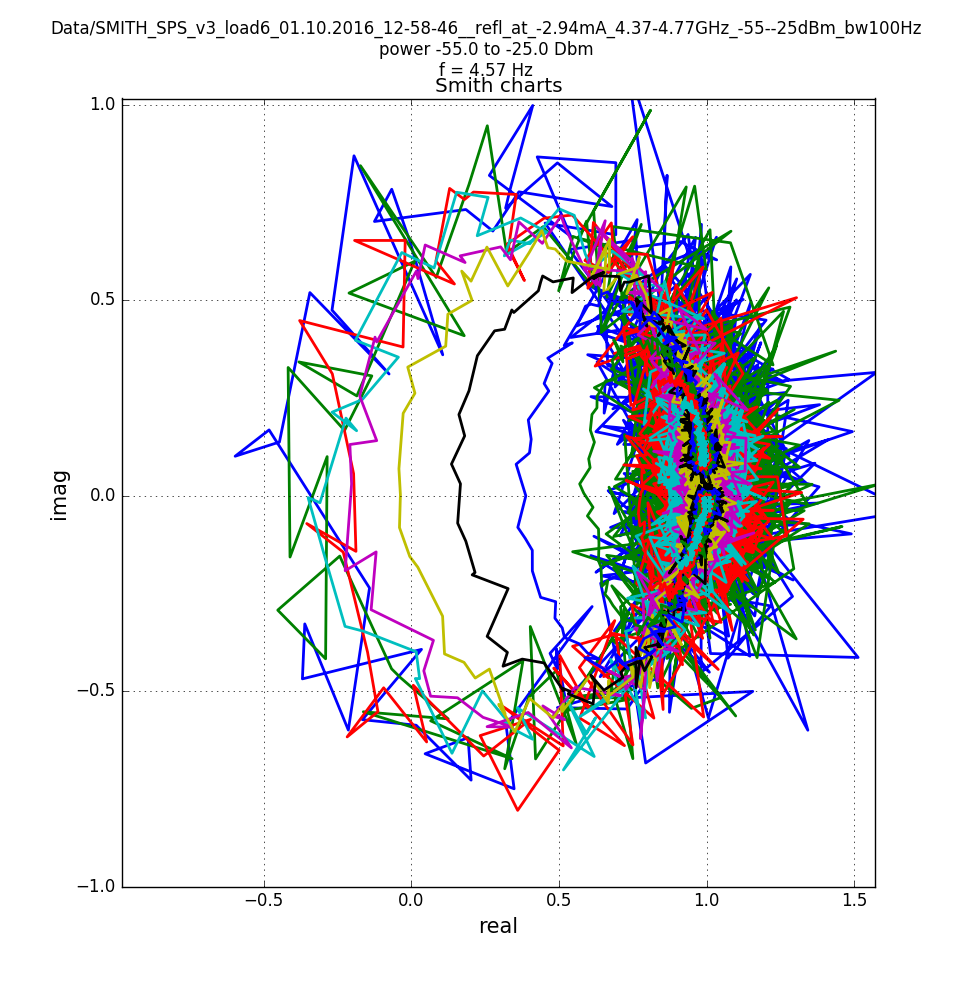
\includegraphics[width=0.8\textwidth]{SMITH_SPS_ver3_load6.png}
	\caption[Зависимость $r_e(\delta\omega)$, измеренная с помощью ВАЦ]{Зависимость $r_e(\delta\omega)$ для различных значений $\Omega$ потокового кубита, измеренная с помощью ВАЦ. Полученное в эксперименте значение $\left. r_e(0)\right\vert_{\Omega=0}\approx-0.4$ характеризует полную эффективность генерации одиночных фотонов как $\Gamma^e_1/2\Gamma_2 \approx 0.7$, что находится в соответствии с результатом \cite{peng2016tuneable}. }
	\label{fig: eff}
\end{figure}
Данное выражение весьма удобно для характеризации внутренних нерадиационных потерь и потерь, возникающих из-за чистой дефазировки. В самом деле, $\Gamma_2 = \Gamma_1/2 + \gamma_\phi $, а это означает, что в наиболее идеальном случае, когда $\Gamma_1^c \ll \Gamma_1^e$, $\Gamma_1^{\text{nr}}=0$~и~$\gamma_\phi=0$, зависимость $r_e(\delta\omega)$ представляется окружностью на комплексной плоскости с центром в точке $(0,0)$ и радиусом 1. В частности, удобно обратить внимание на значение $r_e(0)=-1$ в идеальном случае и не доходящим до этого значения из-за внутренних потерь на кубите. Экспериментально измеренная зависимость $r_e(\delta\omega)$ приведена на Рис.~\ref{fig: eff}. Из измерений можно заключить, что эффективность кубита в качестве источника фотонов составляет примерно 70\%. 

Дополнительно была измерена зависимость $|t_{\text{ce}}(\delta\omega)|$ при различных значениях $\Omega$. Результаты этих измерений приведены на Рис.~\ref{fig: sps_peak_from_power}. Интересно, что выражение для $t_{\text{ce}}$ совпадает с выражением \eqref{eq: refl} для амплитудного коэффициента отражения кубита в линии с точностью до сомножителя $C_c/C_e$. Поэтому данные на Рис.~\ref{fig: sps_peak_from_power} хорошо воспроизводят построенную на Рис.~\ref{fig: refl} зависимость для $|r|$. 
\begin{figure}[h]
	\centering
	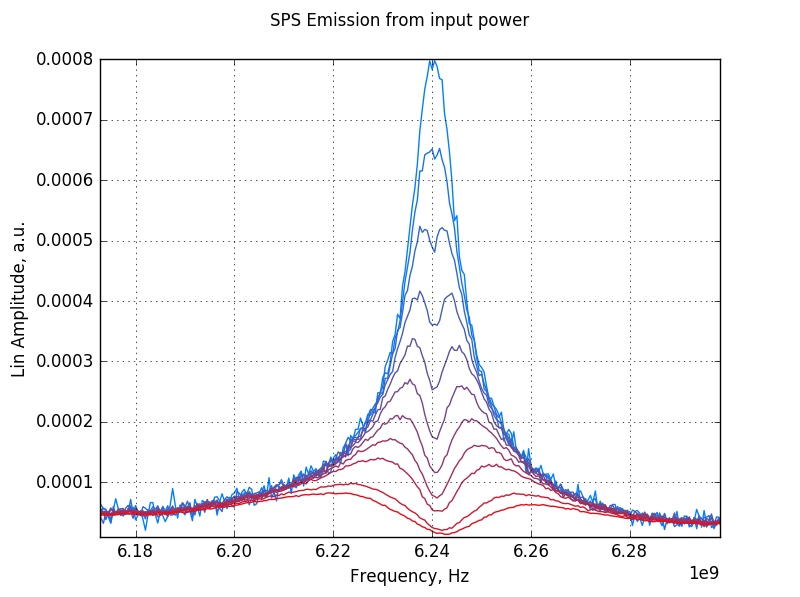
\includegraphics[width=0.8\textwidth]{SPS_peak_from_power.png}
	\caption[Зависимость $t_{\text{ce}}(\delta\omega)$, измеренная с помощью ВАЦ]{Зависимость $t_{\text{ce}}(\delta\omega)$, измеренная с помощью ВАЦ для различных значений $\Omega$. Характер зависимости аналогичен $r(\delta\omega)$ для кубита в линии и описывается соотношением \eqref{eq: refl}}
	\label{fig: sps_peak_from_power}
\end{figure}
Генерация одиночных фотонов от источника требует предварительной калибровки $\pi$-импульсов, которые достигают кубита через контрольную линию и переводят его в состояние $\ket{1}$. Сигнал, сгенерированный кубитом во время распада в линию излучения, и будет являться единичным фотоном с экспоненциально затухающей огибающей, и константа ее затухания полностью определяется значением $\Gamma_1^e$. Для того, чтобы измерить профиль этой огибающей, нужно усреднить большое количество единичных временных разверток средней мощности. Таким образом, временная развертка поля после одного $\pi$-импульса, измеренная при помощи высокоскоростного $АЦП$, возводится в квадрат и результат усредняется по множественным реализациям. Поскольку соотношение <<cигнал-шум>> для измерениц излучаемого кубитом поля достаточно мало, то требуется не менее $10^6$ измерений для получения качественной огибающей. Результат измерения средней мощности от времени приведен на Рис.~\ref{fig: photon_exp}.
Из времени затухания однозначно определяется константа релаксации $\Gamma_1^e$.
\begin{figure}[h]
	\centering
	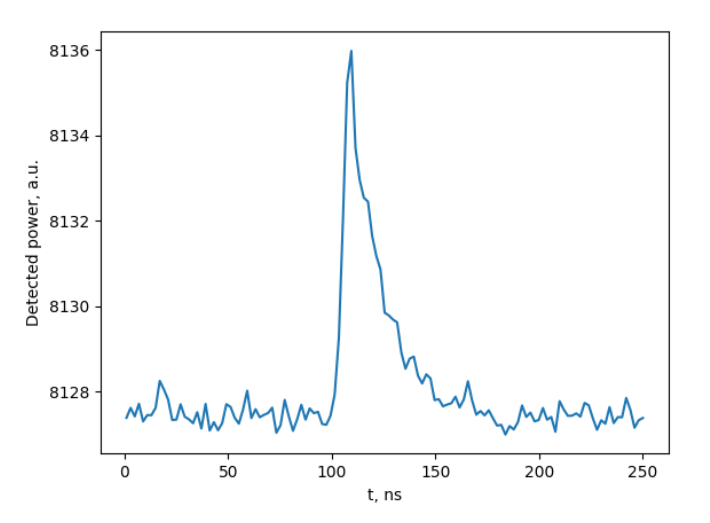
\includegraphics[width=0.6\textwidth]{photon_exp.png}
	\caption[Огибающая одиночного фотона, пропорциональная $\exp(-\Gamma^e_1 t)$]{Огибающая одиночного фотона, пропорциональная $\exp(-\Gamma^e_1 t)$, полученная после $\sim 10^6$ усреднений единичных разверток мощности. Характерное время затухания $1/\Gamma^e_1 \approx 20 $~нс, что соответствует $\Gamma^e_1/2\pi\approx8$~МГц.}
	\label{fig: photon_exp}
\end{figure}
Необходимо отметить, что статистика излучаемого кубитом света будет отличаться от одиночного фотона. Используемая схема подключения кубита к линии излучения --- постоянная емкостная связь --- не позволяет выключать связь с линией во время возбуждения кубита классическим импульсом, поэтому кубит излучает некоторое поле в процессе своего возбуждения, и это поле может иметь не однофотонный характер. Для характеризации статистики излучаемого кубитом поля через измерение корреляционных функций 
\begin{eqnarray}
	&g^{(1)}(\tau) &=\int \braket{V_1(t+\tau)V_2(t)} \,dt, \\
	&g^{(2)}(\tau) &=\int \braket{V_1^2(t+\tau)V_2^2(t)} \,dt.
\end{eqnarray}
была собрана интерференционная схема Хенбери-Брауна-Твисса \cite{confbib1}, изображенная на Рис.~\ref{fig: hbt}. С ее помощью проведены измерения корреляторов первого порядка, см. Рис.~\ref{fig: g1tau}. Корелляторы измерялись при различных последовательности управляющих импульсов: одна из них приводит кубит в состояние $\ket{1}$, а другая --- в состояние $\ket{0+1}/2$. 
\begin{figure}
	\centering
	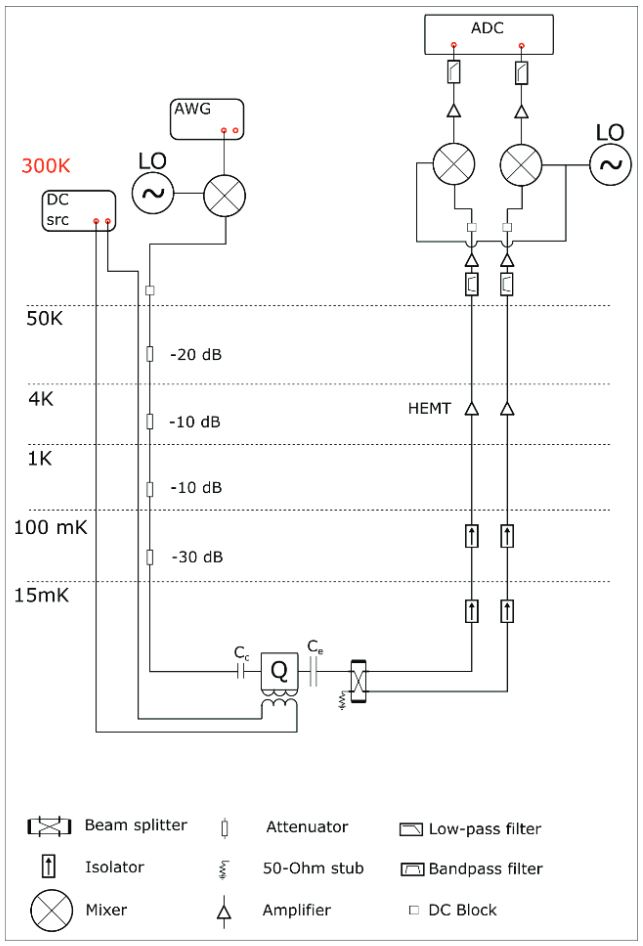
\includegraphics[width=0.5\textwidth]{HBT.jpg}
	\caption[Схема сборки интерферометра Хенбери-Брауна-Твисса]{Схематичное изображение экспериментальной установки, реализующей интерферометрическую схему Хенбери-Брауна-Твисса для излучения от источника одиночных фотонов. Для создания импульсов используется ГИПФ, разведение сигнала по плечам интерферометра осуществляется при помощи гибридного ответвителя, который по своему функционалу аналогичен делителю пучка 50/50 в оптике. Для оцифровки данных используется АЦП.}
	\label{fig: hbt}
\end{figure}
\begin{figure}
	\centering
	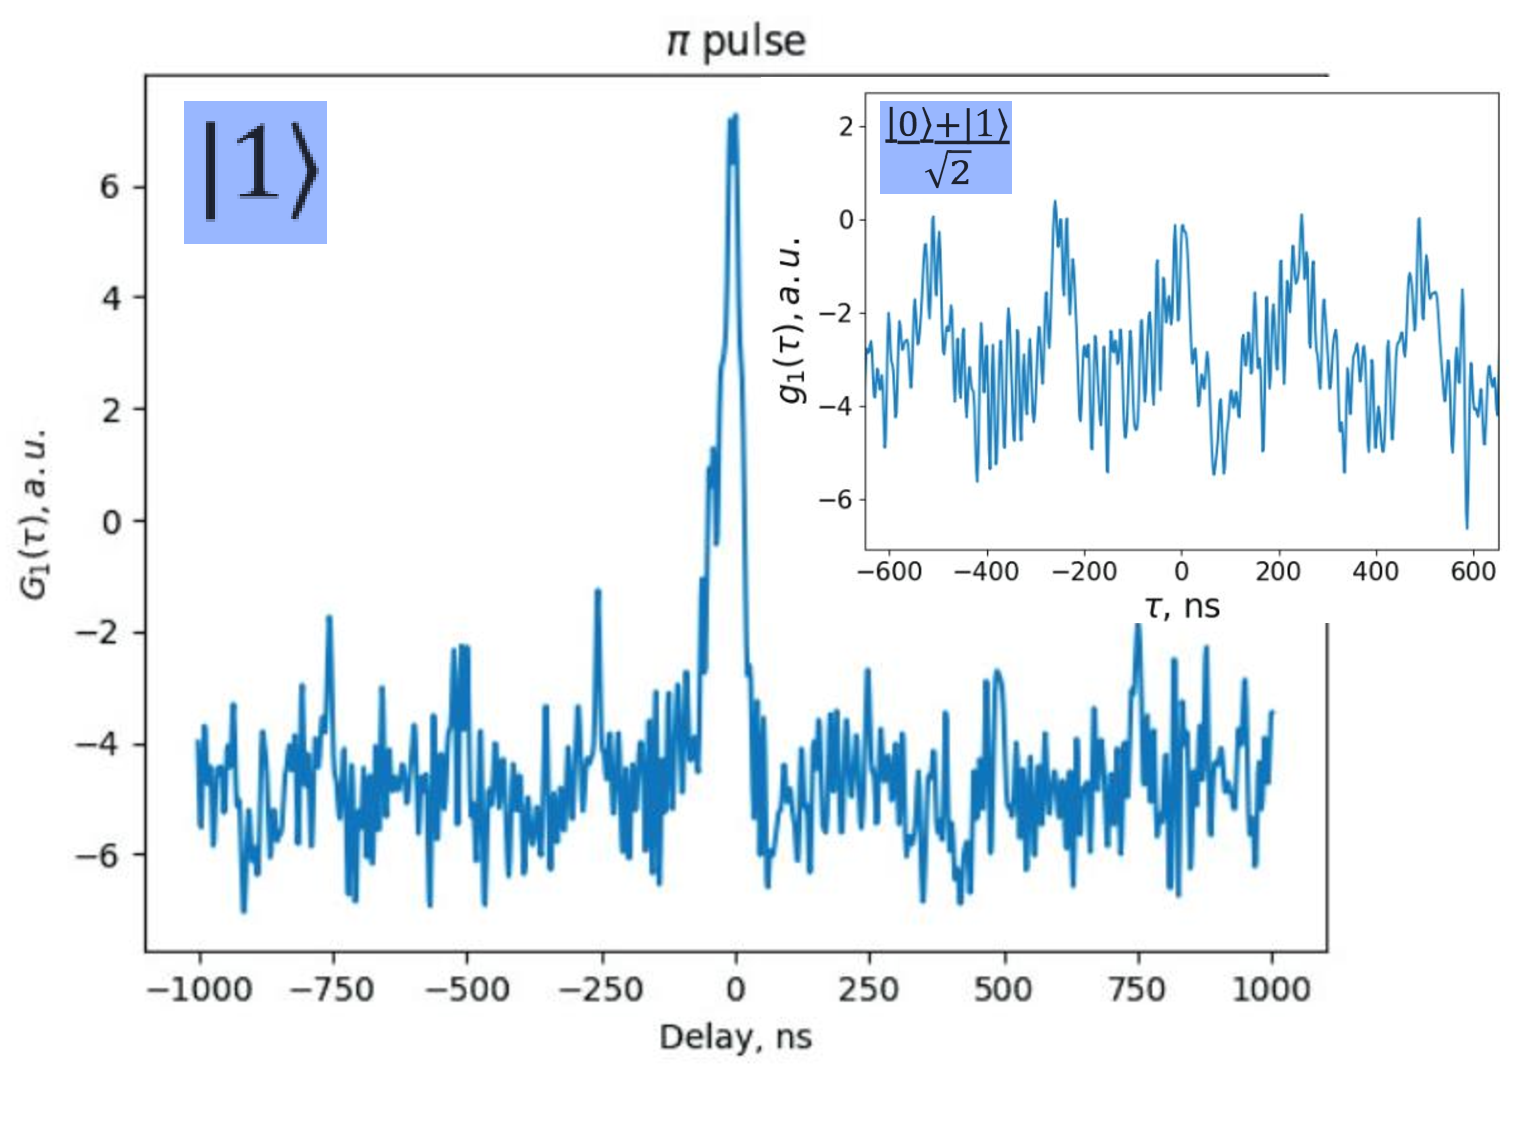
\includegraphics[width=1\textwidth]{G1_meas.pdf}
	\caption[Результаты измерения $g^{(1)}(\tau)$]{Результаты измерения $g^{(1)}(\tau)$ для различных состояний кубита. Отчетливо видно, что для состояния суперпозиции фаза излучения, испускамого кубитом после различных импульсов, корреллирует друг с другом, тогда как для состояния $\ket{1}$ корелляция полей при ненулевой задержке отсутствует.}
	\label{fig: g1tau}
\end{figure}
Отчетливо определяется различный характер корреляций в зависимости от состояния поля в волноводе. Для достоверного определения однофотонности необходимо измерить корреляцию второго порядка для нулевой задержки, чтобы в случае одиночного фотона пронаблюдать полную антикорреляцию, свидетельствующую о том, что фотон целиком летит либо в первое, либо во второе плечо интерферометра. Однако, это измерение предъявляет значительные технические требования, в частности, усреднение как минимум $10^{10}$ отдельных актов испускания фотона, что требует использование ПЛИС для анализа данных, либо же гораздо менее шумящих параметрических усилителей, работающих в квантовом пределе шумов. В рамках этой работы измерение корреляционной функции второго порядка не производилось, однако, в дальнейшем планируется реализация такого измерения.

В завершение данной главы, приведем результаты экспериментального исследования расщепления Аутлера-Таунса для потокового кубита, асимметрично связанного с двумя полупространствами. 

\section{Расщепление Аутлера-Таунса}
Как было подробно рассмотрено в разделе \ref{sec: qo3ls}, для наблюдения расщепления собственных уровней системы из-за взаимодействия с полем необходимо направить на атом резонансную с одним из переходов накачку и наблюдать прохождение слабого пробного сигнала на частоте другого перехода. Результат таких измерений в двух возможных конфигурациях приведен на Рис.~\ref{fig: sps_ats}. Коэффициент прохождения для пробного сигнала вблизи частоте перехода $\ket{0}\leftrightarrow\ket{1}$ ($\ket{1}\leftrightarrow\ket{2}$) значительно меняется при увеличении амплитуды накачки $\Omega$ на частоте перехода $\ket{1}\leftrightarrow\ket{2}$ ($\ket{0}\leftrightarrow\ket{1}$). Дополнительно охарактеризовать возникновение расщепления можно при помощи измерения пропускания при нулевой отстройке, и результаты этих измерений приведены на Рис.~\ref{lines}. Расщепление уровней $\ket{0}$ и $\ket{1}$ приводит к тому, что мощность когеретного поля, излучаемого точно в резонанче с переходом $\ket{1} \leftrightarrow \ket{2}$, значительно падает. Максимум этой мощности практически точно совпадает с условием $\Omega_01 = \Gamma_1^{01}$, отмеченного на Рис.~\ref{lines} оранжевой вертикальной линией, положение которой определено независимо из осцилляций Раби. Таким образом, мы получаем своеобразную версию критерия Релея: свидетельством расхождения пиков на расстояние, большее их относительной ширины $\sim \Gamma_1$, является достижение максимума резонансно излучаемого поля и его последущее спадание при дальнейшем увеличении мощности. 
\begin{figure}[h]
	\centering
	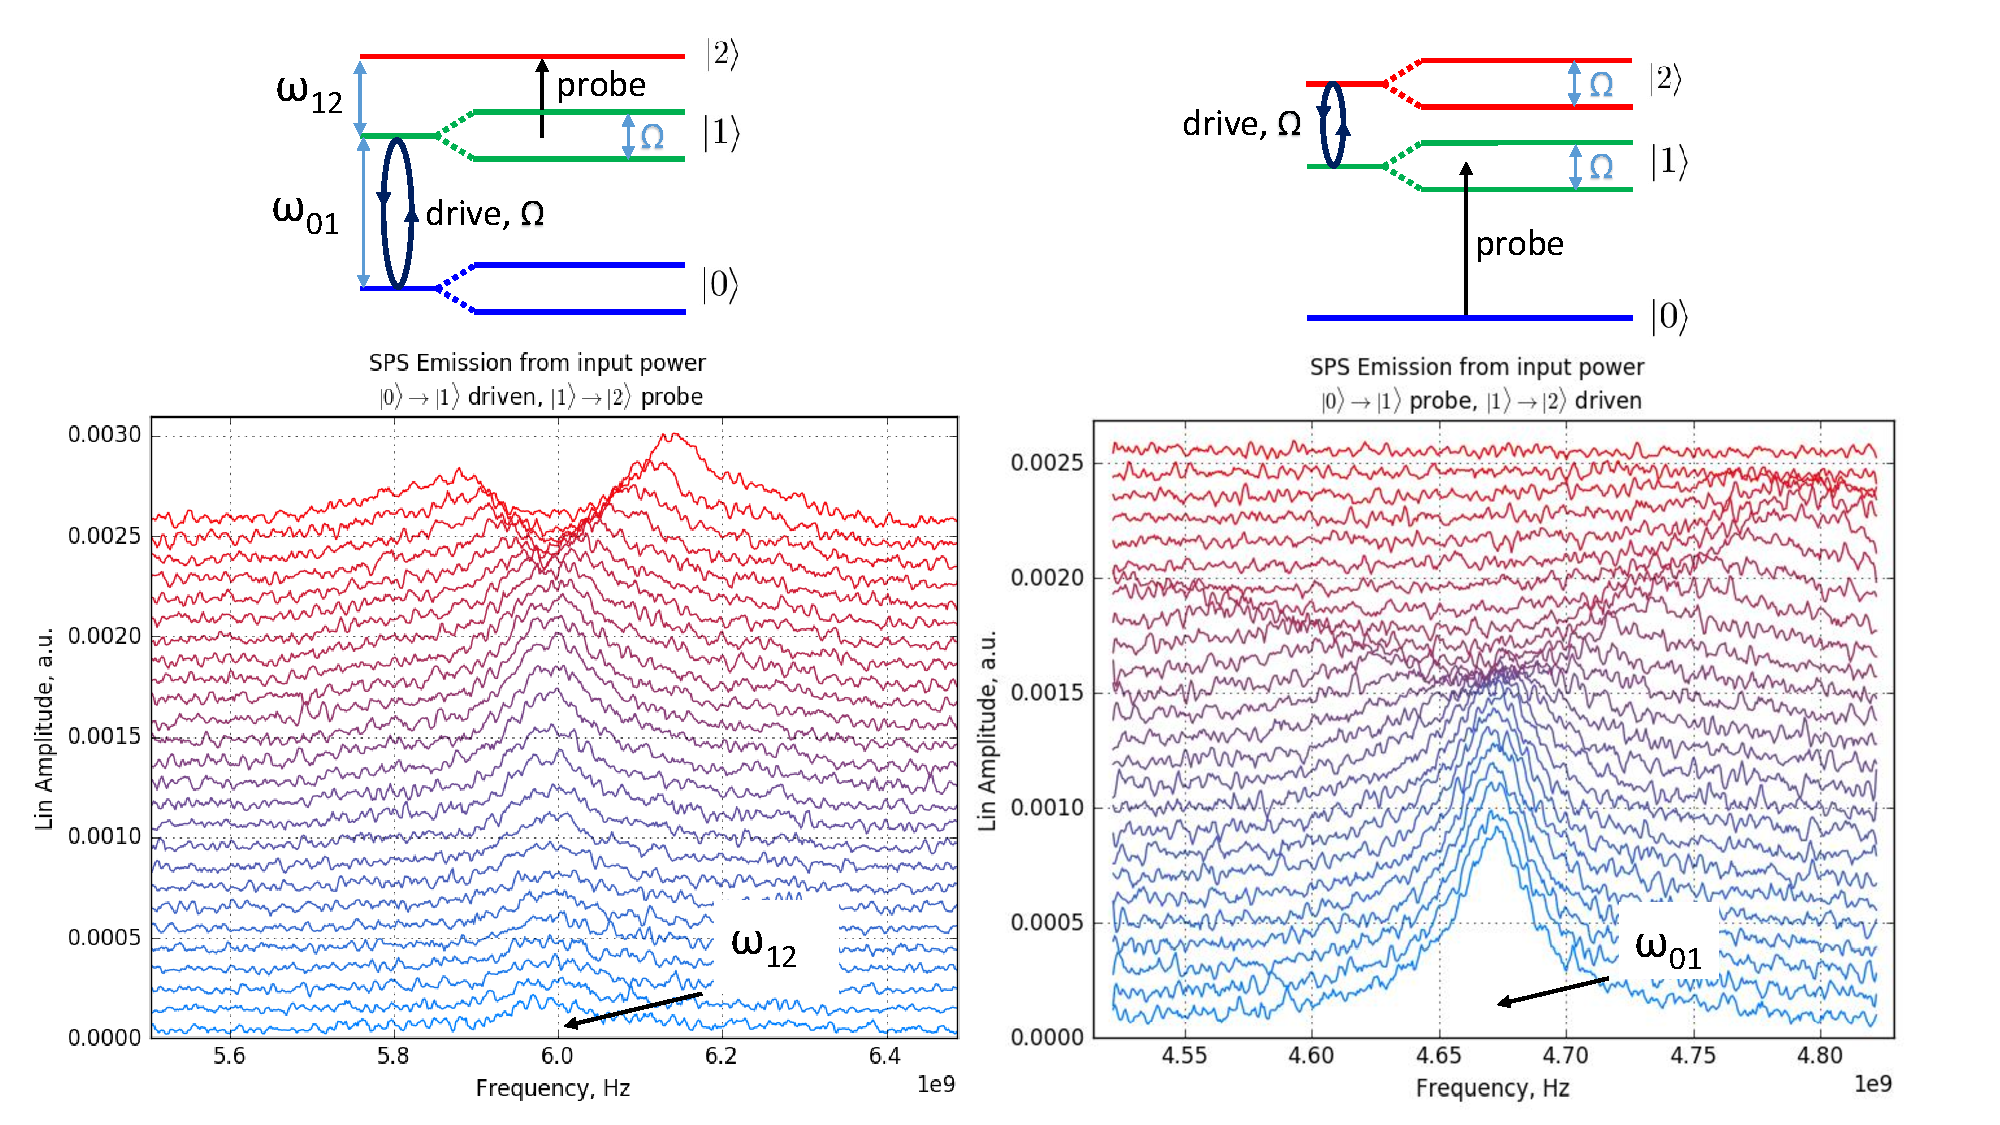
\includegraphics[width=1\textwidth]{SPS_ATS.pdf}
	\caption[Расщепления Аутлера-Таунса в асимметрично связанном потоковом кубите.]{Расщепления Аутлера-Таунса в асимметрично связанном потоковом кубите. Кривые для различных значений мощности сдвинуты по вертикали друг относительно друга.}
	\label{fig: sps_ats}
\end{figure}
\begin{figure}[!ht] 
	\centering
	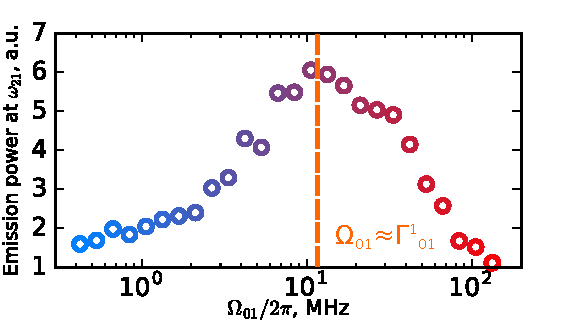
\includegraphics[width=0.7\textwidth]{figure_4-2.pdf} 
	\caption[Зависимость излучения на частоте перехода $\ket{1}\leftrightarrow \ket{2}$ от мощности первого тона на частоте перехода $\ket{0}\leftrightarrow \ket{1}$]{Зависимость излучения на частоте перехода $\ket{1}\leftrightarrow \ket{2}$ от мощности первого тона на частоте перехода $\ket{0}\leftrightarrow \ket{1}$. Оптимальная накачка (наибольшее излучение) соответствует случаю $\Omega_{01} \approx \Gamma_1^{01}$.}
	\label{lines}
\end{figure} 

В данной главе приведены результаты исследования одиночного сверхпроводникового потокового кубита, связанного с двумя полупространствами несимметричным образом. Во-первых, мы продемонстрировали новый способ спектроскопии искусственных атомов, основанный на разделении возбуждающей и излученной волны благодаря асимметричной связи атома с двумя линиями с открытыми концами. Когерентное излучение детектируется со стороны считывающей линии, тогда как атом управляется со стороны более слабо связанной линией контроля. Используя эту методику, мы измерили спектр трёхуровневой системы и определили её времена релаксации. Этот метод будет полезен для приложений в микроволновой квантовой оптике на чипах. Также мы исследовали образец в режиме генерации одиночных фотонов и состояний суперпозиции, в частности, определили эффективность генерации при помощи измерения коэффициента отражения сигнала от кубита, а также измерили огибающую одиночных фотонов во времени и корелляционные функции первого порядка. Эти результаты послужат заделом к созданию более эффективных источников одиночных фотонов и их использованию в комбинированных схемах с большим количеством атомов и волноводов на чипе, что откроет путь для реализации когерентной квантовой СВЧ-электроники на сверхпроводниковых квантовых цепей.